\documentclass[12pt]{article}

\usepackage{fullpage}
\usepackage{graphicx, rotating, booktabs} 
\usepackage{times} 
\usepackage{natbib} 
\usepackage{indentfirst} 
\usepackage{setspace}
\usepackage{grffile} 
\usepackage{hyperref}
\usepackage{adjustbox}
\setcitestyle{aysep{}}


\singlespace
\title{
\textbf{Testing the Public Goods Theory of Alliances}
	}
\author{Joshua Alley\footnote{Graduate Student,
Department of Political Science, Texas A\&M University.}}
\date{{\normalsize \today}}

\bibliographystyle{apsr}

\begin{document}

\maketitle 

\doublespace



%----------------------------------
\section{Other Estimates of Panel Data Interaction}


\subsection{Alternative Estimators}

Robust regression is appropriate for residuals from the growth variable. 
Several observations of states during war see gigantic increases in spending--- the largest value is 140, relative to a median of .063. 
This generates extremely heavy-tailed residuals, so OLS is inefficient. 


Even after applying the inverse hyperbolic sine transformation, the residuals in \autoref{fig:res-qq-plot} deviate strongly from normality. 
\autoref{fig:res-qq-plot} shows the residuals from models 2 and 3 of \autoref{tab:ols-est}, which reports some robustness checks.

\begin{figure}[htbp]
	\centering
		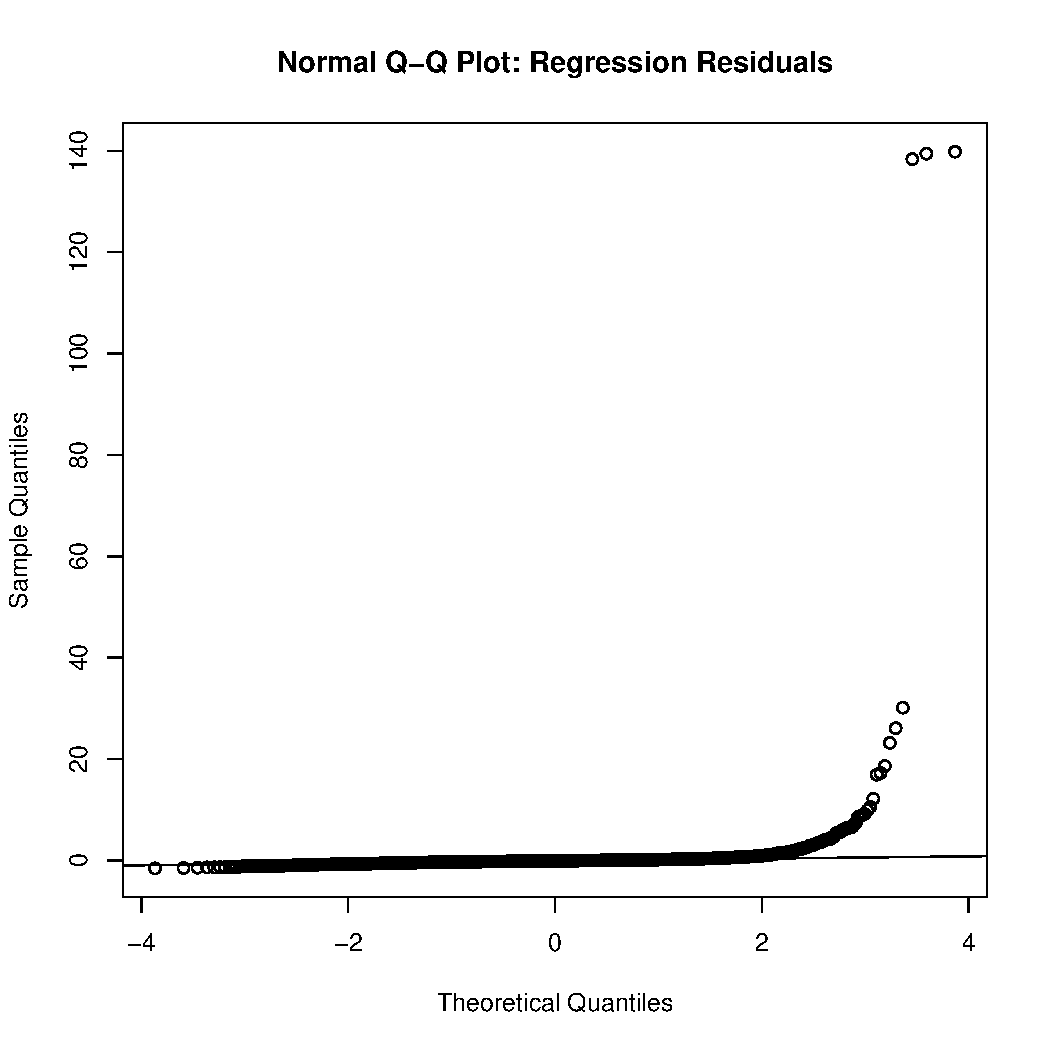
\includegraphics[width=0.95\textwidth]{res-qq-plot.pdf}
	\caption{Plot of residuals against normal quantiles. Deviations from the straight line are deviations from the normal distribution.}
	\label{fig:res-qq-plot}
\end{figure}



Although OLS is not the best estimator for the spending growth data, it produces similar results.
\autoref{tab:ols-est} summarizes estimates from OLS models with and without a transformed growth and spending and robust regression with transformed spending. 

\begin{table}[!htbp] \centering 
\begin{tabular}{@{\extracolsep{5pt}}lccc} 
\\[-1.8ex]\hline 
\hline \\[-1.8ex] 
 & \multicolumn{3}{c}{\textit{Dependent variable:}} \\ 
\cline{2-4} 
\\[-1.8ex] & Growth Spending & \multicolumn{2}{c}{IHS(Growth Spending)} \\ 
\\[-1.8ex] & \textit{OLS} & \textit{OLS} & \textit{Robust Reg.} \\ 
\\[-1.8ex] & (1) & (2) & (3)\\ 
\hline \\[-1.8ex] 
 Change Allied Spending & $-$0.235 & $-$0.099 & $-$0.026 \\ 
  & (0.648) & (0.087) & (0.047) \\ 
  & & & \\ 
 ln(GDP) & $-$0.038$^{**}$ & $-$0.008$^{***}$ & 0.0003 \\ 
  & (0.017) & (0.002) & (0.001) \\ 
  & & & \\ 
 Change Allied Spending $\times$ ln(GDP) & 0.011 & 0.005 & 0.002 \\ 
  & (0.027) & (0.004) & (0.002) \\ 
  & & & \\ 	
 Average Alliance Size & $-$0.003 & $-$0.0001 & 0.0003$^{*}$ \\ 
  & (0.002) & (0.0003) & (0.0002) \\ 
  & & & \\ 
 Average Alliance Democracy & $-$0.001 & $-$0.001 & $-$0.0003 \\ 
  & (0.008) & (0.001) & (0.001) \\ 
  & & & \\ 
 International War & 0.476$^{***}$ & 0.228$^{***}$ & 0.096$^{***}$ \\ 
  & (0.141) & (0.019) & (0.010) \\ 
  & & & \\ 
 Civil War Participant & 0.206$^{**}$ & 0.025$^{*}$ & 0.001 \\ 
  & (0.104) & (0.014) & (0.008) \\ 
  & & & \\ 
 Polity & 0.001 & 0.0001 & $-$0.0001 \\ 
  & (0.005) & (0.001) & (0.0004) \\ 
  & & & \\ 
 External Threat & 0.107 & 0.080$^{***}$ & 0.042$^{***}$ \\ 
  & (0.152) & (0.021) & (0.011) \\ 
  & & & \\ 
 Cold War & 0.032 & 0.034$^{***}$ & 0.047$^{***}$ \\ 
  & (0.058) & (0.008) & (0.004) \\ 
  & & & \\ 
 Constant & 1.074$^{***}$ & 0.259$^{***}$ & 0.026 \\ 
  & (0.413) & (0.056) & (0.030) \\ 
  & & & \\ 
\hline \\[-1.8ex] 
Observations & 9,139 & 9,139 & 9,139 \\ 
R$^{2}$ & 0.003 & 0.025 &  \\ 
Residual Std. Error (df = 9128) & 2.649 & 0.358 & 0.157 \\ 
\hline 
\hline \\[-1.8ex] 
\textit{Note:}  & \multicolumn{3}{r}{$^{*}$p$<$0.1; $^{**}$p$<$0.05; $^{***}$p$<$0.01} \\ 
\end{tabular} 
\caption{Robustness checks of conditional relationship between allied spending, GDP and growth in military spending. }
\label{tab:ols-est}
\end{table} 


The OLS model is a poor fit for the dependent variable. 
The R$^2$ is miniscule, and the standard error of the residual is much larger than the robust regression. 
Transforming the DV improves the performance of OLS, but leads to similar inferences. 
Despite the lackluster fit, I present these results to show that the conventional estimator generates similar inferences. 


Rather than interpret the coefficients, I plot the marginal effect of allied spending across the range of GDP for these three models.
\autoref{fig:me-plots} compares these results with the marginal effects plot from the robust regression in the paper. 
Three of the four estimation strategies produce a positive marginal effect, along with broad enough confidence intervals to suggest a conditional relationship with GDP is unlikely.\footnote{The robust regression results are so similar because even after transforming spending growth, the robust estimator down-weights those extreme observations a great deal.} 
OLS without a transformed DV finds no positive impact of changing allied capability on growth in spending, but this result should be taken with great caution due to poor model fit. 
Regardless, none of the results matches the expectation of a negative effect which increases in state size. 


\begin{figure}[htbp]
	\centering
		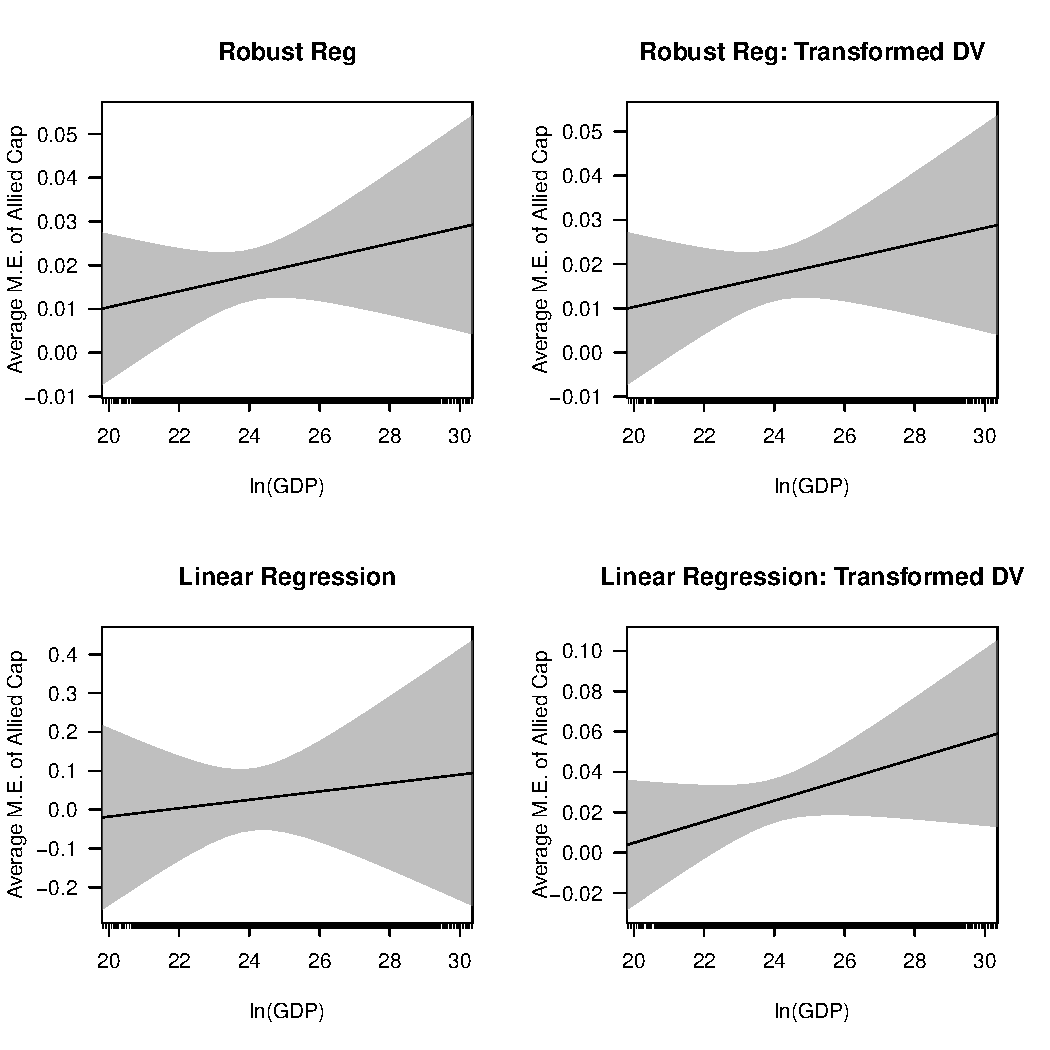
\includegraphics[width=0.95\textwidth]{me-plots.pdf}
	\caption{Comparison of marginal effect of changing allied spending on growth in military spending across the range of GDP. Each plot corresponds to an estimation strategy.}
	\label{fig:me-plots}
\end{figure}



I also checked whether inferences were sensitive to non-random selection into alliances. 
I employed a Heckman selection model, where the second-stage estimation sample was states in alliances. 
The second-stage model used the same specification as the robust regression.


A first-stage probit model predicts the presence of at least one alliance. 
The first stage model includes lagged levels of military spending, the log of GDP, regime type, international conflict, and external threat as covariates. 
\autoref{tab:heckit-res} summarizes the output of the second-stage equation.  


\begin{table}[!htbp] \centering 
\begin{tabular}{@{\extracolsep{5pt}}lc} 
\\[-1.8ex]\hline 
\hline \\[-1.8ex] 
 & Growth Military Spending \\ 
\hline \\[-1.8ex] 
 Change Allied Spending & $-$0.304 \\ 
  & (0.266) \\ 
  & \\ 
 ln(GDP) & 0.201$^{***}$ \\ 
  & (0.017) \\ 
  & \\ 
 Change Allied Spending $\times$ ln(GDP) & 0.013 \\ 
  & (0.011) \\ 
  & \\ 
 International Conflict & 0.362$^{***}$ \\ 
  & (0.140) \\ 
  & \\ 
 Civil War Participant & 0.005 \\ 
  & (0.049) \\ 
  & \\ 
 POLITY & $-$0.022$^{***}$ \\ 
  & (0.004) \\ 
  & \\ 
 External Threat & $-$0.098 \\ 
  & (0.151) \\ 
  & \\ 
 Cold War & 0.102$^{***}$ \\ 
  & (0.026) \\ 
  & \\ 
 Constant & $-$5.443$^{***}$ \\ 
  & (0.416) \\ 
  & \\ 
\hline \\[-1.8ex] 
Observations & 9,235 \\ 
\hline 
\hline \\[-1.8ex] 
\textit{Note:}  & \multicolumn{1}{r}{$^{*}$p$<$0.1; $^{**}$p$<$0.05; $^{***}$p$<$0.01} \\ 
\end{tabular} 
\caption{Heckman Sample Selection Regression Estimates: Allied Spending, GDP, and Growth in military spending 1816-2007.}
\label{tab:heckit-res}
\end{table} 

In the selection model, change in allied spending has no association with growth in spending. 
GDP is positively associated with military expenditures, but the interaction term remains statistically insignificant. 
Even after accounting for non-random selection into alliances, there is little evidence of a conditional relationship between alliance spending and state size. 
 

\subsection{Continuous modifying Variable}


\citet{Hainmuelleretal2019} show linearity assumptions and a lack of support in the range of the modifying variable can generate misleading inferences in interactive models. 
They suggest estimating associations with binning and kernel estimators to check for non-linearity and adequate support. 
\autoref{fig:inter-bin-abs} plots the results of the binning estimator. 


\begin{figure}
	\centering
		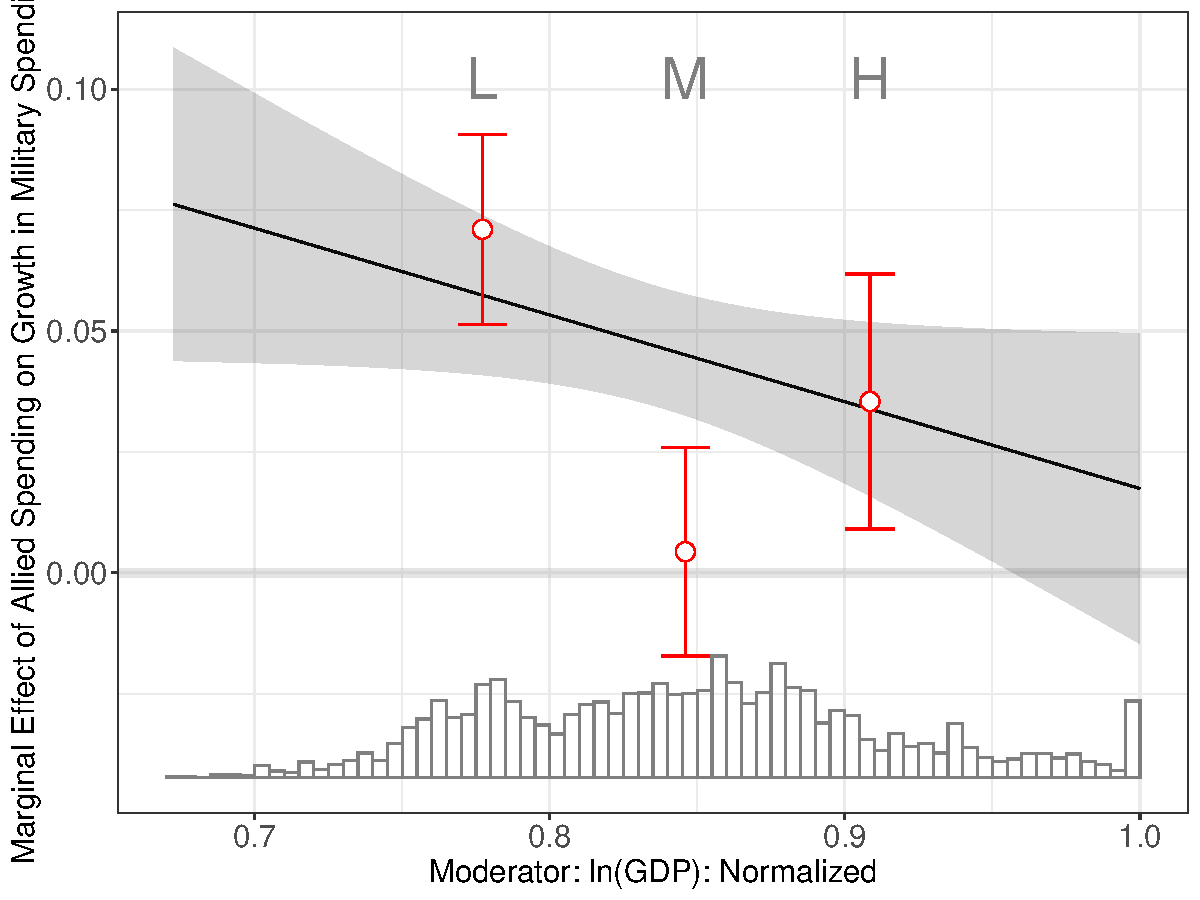
\includegraphics[width=0.95\textwidth]{inter-bin-abs.pdf}
		\caption{Binning estimates of interaction between changes in allied spending and GDP.}
	\label{fig:inter-bin-abs}
\end{figure}


The binning estimator suggests that the linearity assumptions of the robust regression are acceptable. 
There is still no evidence state size modifies the impact of allied spending on growth in military spending, however. 
The marginal effect of allied spending cannot be distinguished from zero across the range of GDP. 


\begin{figure}
	\centering
		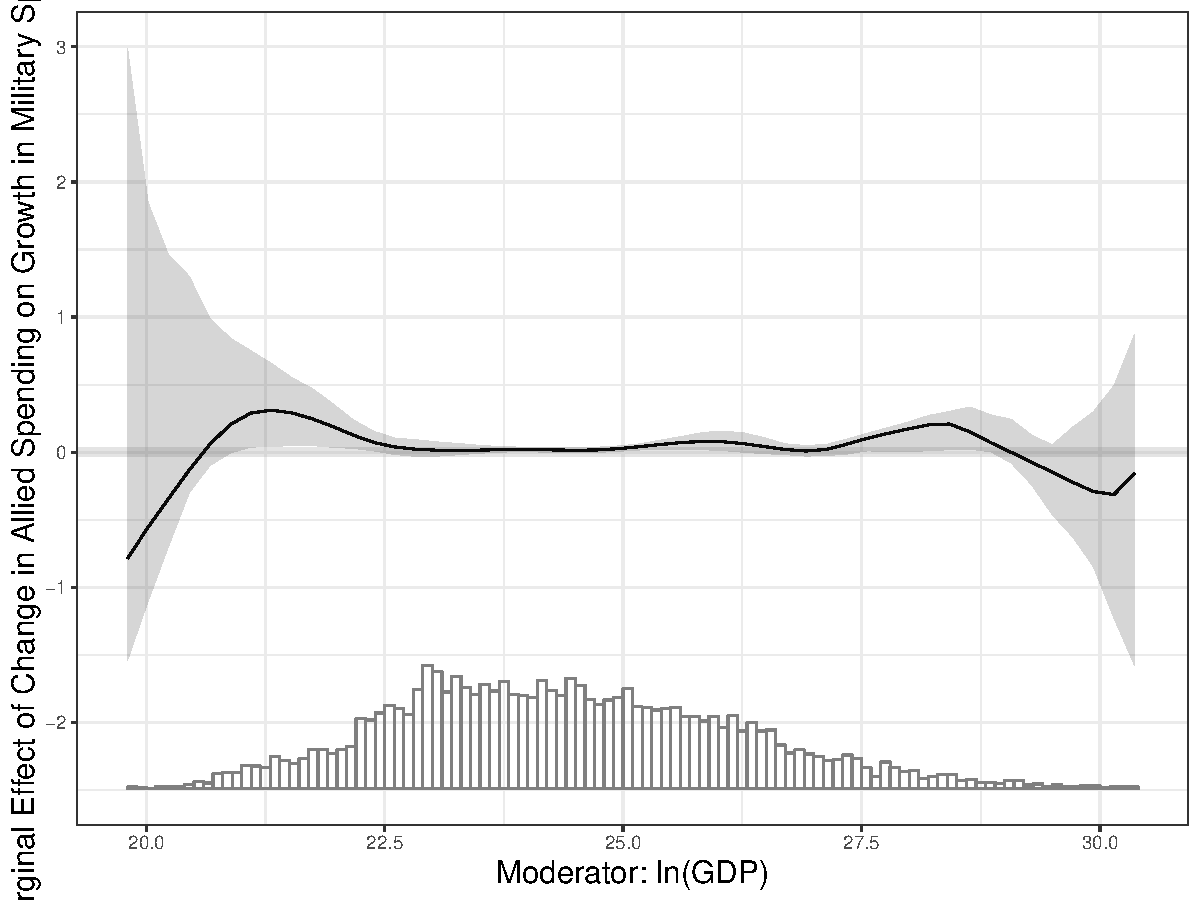
\includegraphics[width=0.95\textwidth]{inter-kernel-abs.pdf}
	\caption{Kernel estimate of interaction between changes in allied spending and GDP.}
	\label{fig:inter-kernel-abs}
\end{figure}


The kernel estimator also generates little evidence of a conditional relationship. 
As \autoref{fig:inter-kernel-abs} demonstrates, the marginal effect of spending is mostly positive. 
Negative point estimates of the marginal effect are indistinguishable from zero. 
Relaxing the linearity assumptions of the robust regression does little to change substantive inferences about the presence of a conditional relationship. 




\section{Alternative Sample for Multilevel Model}


It is possible that estimating a model on the full sample of states makes misleading comparisons by including states with no alliances.
Without protection from an alliance, these states might have to spend more on the military \citep{Morrow1993}. 
Increasing contribution would have less of an impact compared to these countries than to other states in alliances. 


To check whether this was the case, I re-fit the multilevel model on a sample of only states with at least one alliance. 
This reduced the sample size from 9,961 observations to 6,148. 
The results are relatively unchanged, however. 


138 treaties have a positive mean $\gamma$ parameter, and 18 of those treaties have a 90\% credible interval that excludes zero. 
147 treaties have a negative mean $\gamma$ estimate, and 15 of those treaties have a 90\% credible interval that excludes zero.
Thus the prediction success rate for a public goods model increases marginally from 5.6\% in the full sample to 6.3\%  in a sample with only alliance participants. 
This is not a large enough change to suggest the results are qualitatively different. 


Furthermore, as \autoref{fig:sample-comp-gamma} shows, the distribution of the association between treaty contribution and spending across alliances is very similar across the two samples. 
This figure overlays the distribution of the mean $\gamma$ parameters in each sample. 
The is little discernible difference between the two. 


\begin{figure}
	\centering
		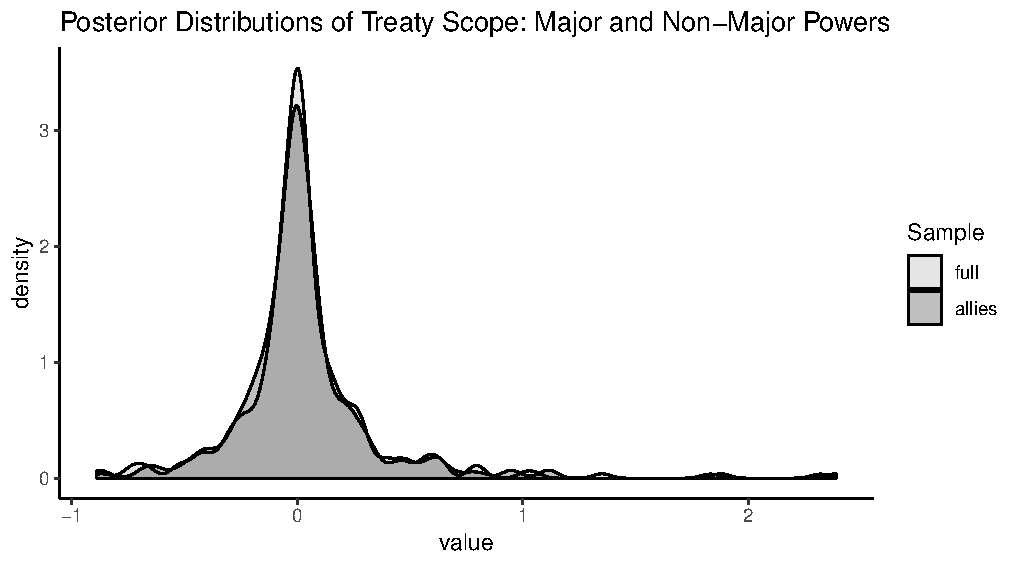
\includegraphics[width=0.95\textwidth]{sample-comp-gamma.pdf}
	\caption{Comparison of the distribution of $\gamma$ parameters in full sample and a sample of only alliance participants. There is minimal different in the distribution of these parameters across the two samples.}
	\label{fig:sample-comp-gamma}
\end{figure}






\section{Convergence of Multilevel Model} 


There were no divergent iterations in sampling, which would have invalidated the results. 
However, there are other threats to inference from the posterior samples. 
Given heavy tails in military spending growth, STAN might have struggled to explore the posterior distribution. 


Energy plots can diagnose this problem. 
\autoref{fig:energy-plot} plots the marginal energy distribution and the first differenced distribution. 
If the two histograms do not overlap, sampling was impeded by heavy tails. 
The substantial overlap in the distributions for all four chains in \autoref{fig:energy-plot} indicates this was not a problem. 


\begin{figure}
	\centering
		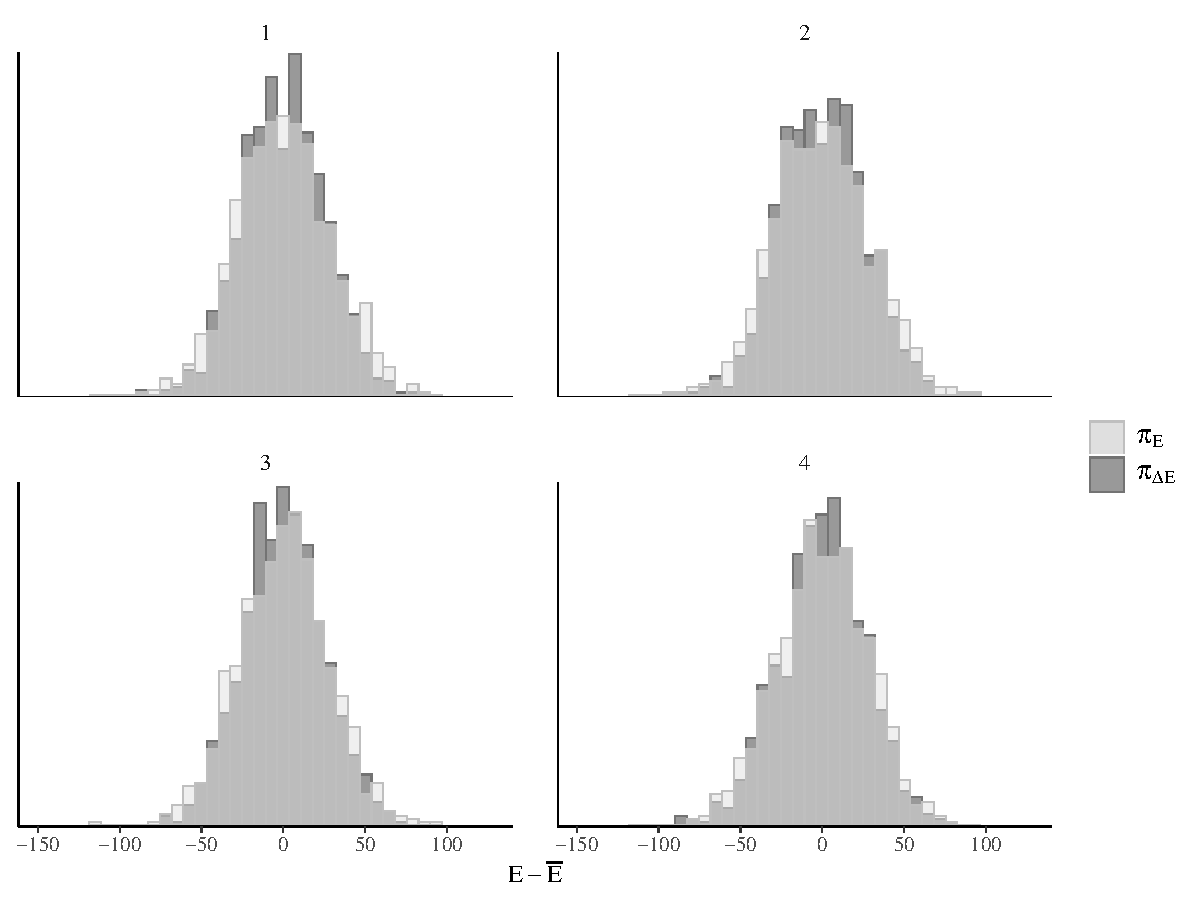
\includegraphics[width=0.95\textwidth]{energy-plot.pdf}
	\caption{Energy plot of multilevel model results. Greater overlap in the two histograms indicates adequate exploration of the posterior distribution. }
	\label{fig:energy-plot}
\end{figure}


The split $\hat{R}$ statistic is another way to assess convergence. 
$\hat{R}$ compares the behavior of each chain by measuring the ratio of the average variance of draws within each chain to the variance of the pooled draws across chains. 
When $\hat{R}$ is close to 1, all the chains have similar variance, and are therefore in equilibrium. 


The standard heuristic is that an $\hat{R}$ greater than 1.1 is problematic. 
\autoref{fig:rhat-plot} plots the $\hat{R}$ statistic for every parameter in the model. 
No parameters generate concern, even at a more conservative threshold of 1.05. 


\begin{figure}[htbp]
	\centering
		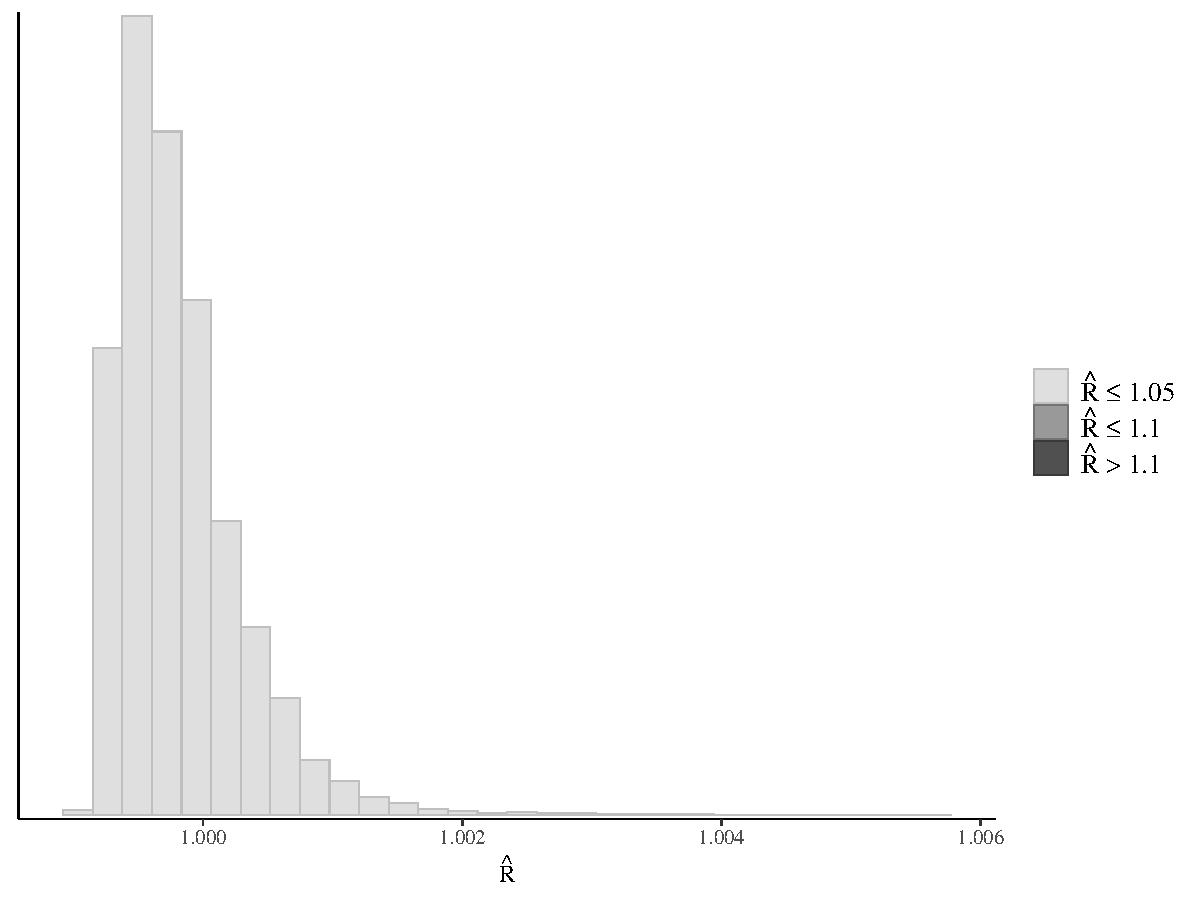
\includegraphics[width=0.95\textwidth]{rhat-plot.pdf}
	\caption{Histogram of split $\hat{R}$ statistic for all parameters in the multilevel model.}
	\label{fig:rhat-plot}
\end{figure}
 


\subsection{Multilevel Model Priors} 

All priors are specified to be weakly informative relative to the scale of the data \citep{Gelmanetal2017}. 
I summarize the prior distributions for each set of parameters in \autoref{tab:priors}. 
$p(nu)$ a well-behaved prior for the degrees of freedom in a t-distribution \citep{JuarezSteele2010}. 
Given that median growth in military expenditures is 0.06, the standard normal priors on the $\beta$ and $\gamma$ parameters are quite diffuse. 


\begin{table} % Create a table of priors.
\begin{center}
\begin{tabular}{c} 
$ p(\alpha) \sim N(0, 1)$  \\
$ p(\sigma) \sim \mbox{half-}N(0, 1) $ \\
$ p(\alpha^{yr}) \sim N(0, \sigma^{yr}) $ \\ 
$ p(\sigma^{yr}) \sim N(0, 1) $ \\
$ p(\alpha^{st}) \sim N(0, \sigma^{st}) $ \\ 
$ p(\sigma^{st}) \sim \mbox{half-}N(0, 1) $ \\ 
$ p(\sigma^{all}) \sim \mbox{half-}N(0, 1) $ \\
$ p(\beta) \sim N(0, 1) $ \\
$ p(\gamma) \sim N(0, 1) $ \\ 
$ p(\nu) \sim gamma(2, 0.1)$ 
\end{tabular} 
\caption{Summary of Priors in Multilevel Model} 
\label{tab:priors}
\end{center} 
\end{table} 


To facilitate estimation, I use a non-centered parameterization for the state and year varying intercepts \citep{BetancourtGirolani2015}. 
The prior is equivalent, but a non-centered parameterization decouples the mean and variance, which makes sampling easier. 
I also employ a sparse matrix representation of the alliance membership matrix $\textbf{Z}$ to speed up estimation. 


\singlespace


\bibliography{../../../MasterBibliography} 





\end{document}
